\documentclass[a4paper,11pt]{article}
%\usepackage[utf8x]{inputenc}
\usepackage[utf8]{inputenc}
\usepackage{graphicx}
\usepackage{booktabs}
\usepackage{lscape}

%opening
\title{Automatic assessment of Computational Thinking in Scratch projects with Dr. Scratch}
\author{Jesús Moreno-León, Gregorio Robles \\ Programamos.es, Sevilla, Spain - Universidad Rey Juan Carlos, Madrid, Spain \\ jesus.moreno@programamos.es, grex@gsyc.urjc.es}

\begin{document}

\maketitle

\begin{abstract}
In this paper we present Dr. Scratch, a web-based tool to automatically assess the development of Computational Thinking of Scratch projects. The paper reviews similar initiatives, like Hairball, and investigates the literature with proposals for assessment of Scratch projects that we have studied and remixed in order to develop the Computational Thinking analysis. Then it introduces the various aspects that Dr. Scratch takes into consideration to compute a Computational Thinking score for a Scratch project and presents some preliminar findings of the analysis of over 100 investigated Scratch projects. Finally, future directions and limitations are presetned and discussed.

\end{abstract}

\section{Introduction}

Computational Thinking (CT) was defined by Wing as a skill that ``involves solving problems, designing systems, and understanding human behaviour, by drawing on the concepts fundamental to computer science''~\cite{wing2006computational}. In the last years, governments and educational institutions around the world are trying to include the development of this competence in schools~\cite{euschoolnet}. In this regard, Lye and Koh, in their 'Review on teaching and learning of computational thinking through programming'~\cite{lye2014review}, show that programming is a key instrument to develop this skill.

However, as explained in Section~\ref{sec:background}, assessing the development of computational thinking is not a trivial issue, and several authors, like Resnick and Brennan, have proposed different strategies and frameworks to try to address the evaluation of this competence~\cite{brennan2012new}. New tools are being developed to assist educators in the assessment of the CT of learners. One of the most relevant tools is Hairball~\cite{boe2013hairball}, a static code analyzer for Scratch projects that detects programming errors in the scripts of the projects.

Dr Scratch~\cite{moreno2014drscratch} is a free/open source web tool, powered by Hairball, that analyzes Scratch projects to automatically assign a CT score in terms of abstraction, logical thinking, synchronization, parallelism, flow control, user interactivity and data representation. Section~\ref{sec:methodology} presents the algorithm used to assess the CT from Scratch code, which has been developed by remixing different proposals of educators and researchers who are using Scratch to teach Computer Science in primary and secondary schools.
Section~\ref{sec:findings} shows the results of analyzing 100 projects we randomly downloaded from the Scratch web repository. Finally, in the conclusions of the paper we discuss the limitations of our approach, as some pillars of CT, such as debugging or remixing skills, cannot be evaluated with this solution.


\section{Background}
\label{sec:background}

The assessment of the development of CT is one of the most discussed topics by educators and researchers in educational conferences, seminars and workshops in the last years. Regarding the Scratch programming language, several authors have proposed different approaches to evaluate the development of CT of a learner by analyzing their Scratch projects. 

Thus, Brennan and Resnick, in their paper ``New frameworks for studying and assessing the development of computational thinking'''~\cite{brennan2012new}, present a strategy based on project portfolio analysis using a visualization tool called Scrape~\cite{wolz2011scrape}, although their proposal is completed with artifact-based interviews and design scenarios.

Wilson, Hainey and Connolly~\cite{wilson2012evaluation} suggest a scheme to gauge the level of programming competence demonstrated by a student by analyzing a project in terms of programming concepts (such as threads, conditional statements or variables), code organisation (variable names, sprite names and extraneous blocks) and designing for usability (like functionality, instructions or originality, among others).

In this line, Seiter and Foreman developed the Progression of Early Computational Thinking Model, a framework to assess CT in primary students coding with Scratch by synthesizing ``measurable evidence from student work with broader, more abstract coding design patterns, which are then mapped onto computational thinking concepts''~\cite{seiter2013modeling}.

In order to assist educators with a tool that could be used to partly automate the assessment of Scratch projects, Boe et al. developed Hairball~\cite{boe2013hairball}, a Lint-inspired static analysis of Scratch projects that detects issues in the code, such as code that is never executed, messages that no object receives or attribute not correctly initialized. This tool was used to asses Computer Science learning in a Scratch-based summer camp~\cite{franklin2013assessment}. 

\section{Methodology}
\label{sec:methodology}

Inspired by the work reviewed in Section~\ref{sec:background}, we developed a plug-in for the Hairball environment, \textit{Mastery}\footnote{https://github.com/jemole/hairball/blob/master/hairball/plugins/mastery.py}, that analyses a Scratch project to assign a CT score depending on the competence demonstrated by the developer on the following seven concepts: abstraction and problem decomposition, logical thinking, synchronization, parallelism, algorithmic notions of flow control, user interactivity and data representation. In order to evaluate the level of development on each of these concepts, the \textit{Mastery} plug-in implements an algorithm based on the rules in Table~\ref{table:CTscore}.

\begin{table*}[t]
\centering
%\begin{tabular}{p{2.5cm}p{2.7cm}p{3cm}p{4cm}}
\begin{tabular}{|l|p{2.7cm}|p{3cm}|p{4cm}|}
%\toprule
\hline
CT concept & Basic & Developing & Proficient\\ %\midrule 
\hline
\hline  
Data representation & modifiers of sprites properties &
operations on vars & operations on lists  \\
\hline
Logical thinking & if & if else & logic operations \\ 
\hline
User Interactivity & green flag & key pressed, sprite clicked, ask and wait,
mouse blocks & when \%s is \textgreater \%s, video, audio \\ 
\hline
Flow control & sequence of blocks & repeat, forever & repeat until \\ 
\hline
Abstraction & more than one script & more than one script and more than one sprite & def block\\
\hline
Parallelism & Two scripts on green flag & Tow scripts on key pressed, two scripts on sprite clicked on the same sprite & Two scripts on when I receive message, create clone, two scripts when \%s is \textgreater \%s, two scripts on when backdrop change to \\
\hline
Synchronization & wait & Broadcast, when I receive message, stop all, stop program, stop programs sprite & wait until, when backdrop change to, when I start as clone, broadcast and wait \\ 
\hline
\end{tabular}
\caption{Level of development for each CT concept.}
\label{table:CTscore}
\end{table*}


Figure~\ref{fig:logic} can be used to illustrate the operation of the plug-in. Thus, following the rules in Table~\ref{table:CTscore}, the first script of the picture would be cataloged as \textit{basic} in terms of logical thinking, as only \textit{if} statements are used. The second script, however, would be considered to demonstrate a \textit{developing} level, because an \textit{if else} block is utilized. Finally, the third script would prove a \textit{proficient} level on this concept, as a logical operation, \textit{or}, is being used.

\begin{figure}
  \centering
    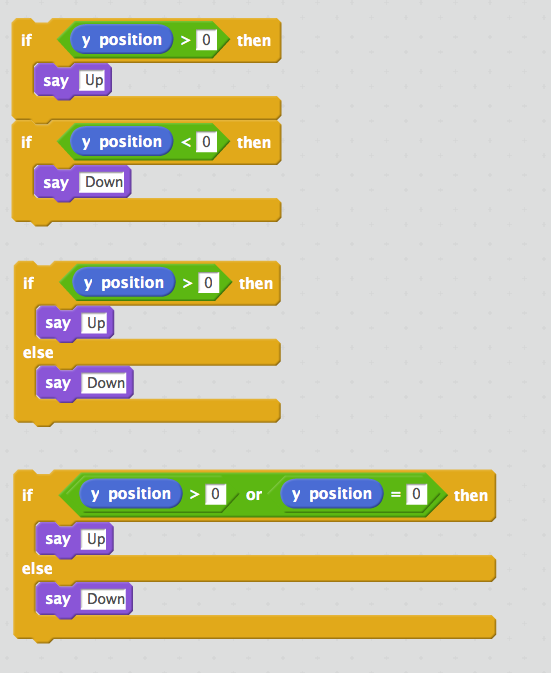
\includegraphics[width=9cm]{img/Logic.png}
    \caption{Different levels of development of logical thinking: basic (top), developing (center) and proficient (bottom).}
    \label{fig:logic}
\end{figure}

With the aim of making it easier for users to analyze their projects, we have developed a web tool called Dr. Scratch\footnote{http://drscratch.programamos.es/} that allows to analyze Scratch programs by either uploading an sb2 file or just introducing the URL of the project. Figure~\ref{fig:drscratch} shows the output of Dr. Scratch tool after performing the analysis on a Scratch project called Just Jump\footnote{http://scratch.mit.edu/projects/52452686/}. An overall CT score of 16 points is computed, informing the user about the partial count of the different CT concepts in a table below. Future versions of Dr. Scratch are planned to provide more information on how to improve each of the aspects where there is room for improvement by the learner.

\begin{figure}
  \centering
    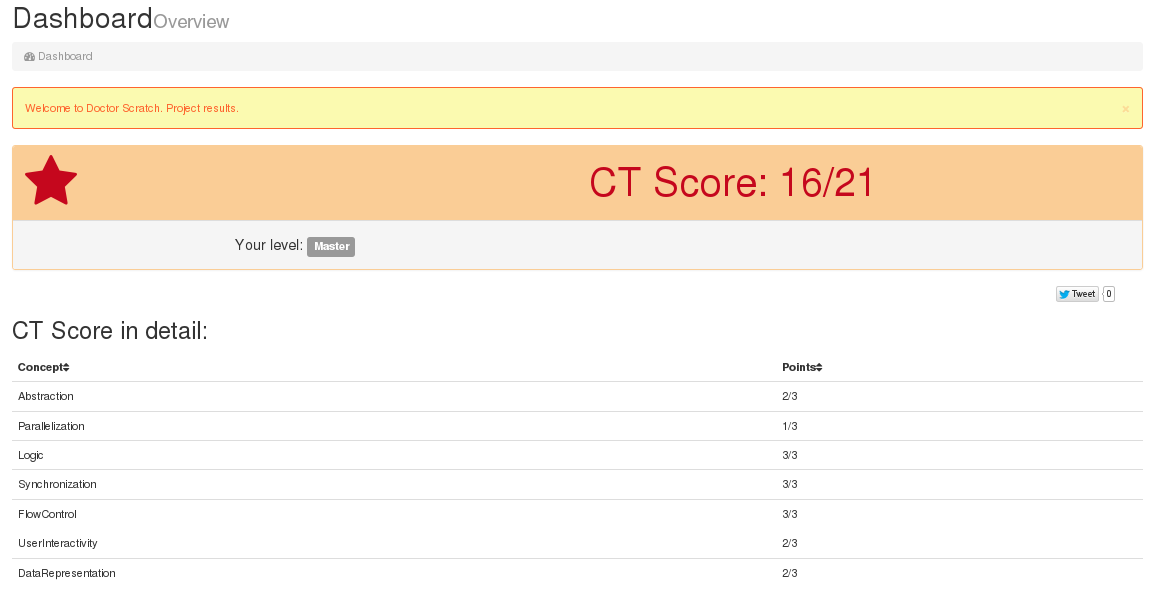
\includegraphics[width=13cm]{img/results.png}
    \caption{Dr. Scratch shows the CT Score after analysing a Scratch project.}
    \label{fig:drscratch}
\end{figure}

\section{Preliminar Findings}
\label{sec:findings}

In order to test the operation of the \textit{Mastery} plug-in, we randomly downloaded and analysed 100 projects from the Scratch repository. The average CT score was 14.4 points, while the median was 16 and the mode 18. As can be seen in figure~\ref{fig:scores}, which presents the mean score for each of the CT components, the concepts in which higher results were obtained are flow control, abstraction, parallelism and synchronization, while user interactivity and data representation got slightly lower values.
\begin{figure}
  \centering
    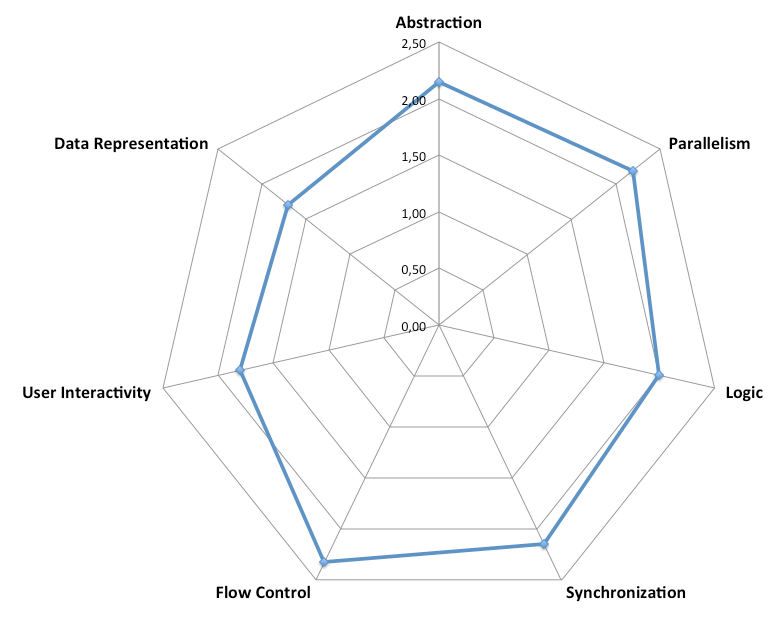
\includegraphics[width=10cm]{img/spider.png}
    \caption{CT score average of 100 randomly downloaded project from the Scratch repository.}
    \label{fig:scores}
\end{figure}

\section{Conclusions and future work}
\label{sec:conclusions}

In this paper we present the procedure used by Dr. Scratch tool in order to assess the development of the CT demonstrated by the developer of a Scratch project. The tool assigns a CT score which is calculated by adding up the partial counts of each CT concept: abstraction, logical thinking, synchronization, parallelism, flow control, user interactivity and data representation.

This approach has several limitations. On the one hand, the examination of a single project might not be as accurate or complete as the analysis of the collection of projects of the user; in this regard, the new feature of Dr. Scratch tool that will allow \emph{scratchers} create an account to store the record of multiple analysis might alleviate this issue. Furthermore, the use of a particular block or groups of blocks is not enough to confirm fluency on a certain CT concept; other plug-ins like \textit{Dead code}, \textit{Attribute initialization}, \textit{Sprite naming} or \textit{Repeated code} have been incorporated to Dr. Scratch tool aiming to detect if the blocks are being used correctly~\cite{moreno2014automatic}. Nevertheless, the bigger limitation of this approach is the fact that some key CT competences cannot be measured by analysing the code of a project, such as the debugging or remixing skills. 

Therefore, this solution must be used by students as a tool to receive feedback that might help them to discover areas in which to focus to keep on improving their coding skills, or by teachers as a tool that might assist them in the assessing of Scratch projects, but not as a replacement of the evaluators work.

In the near future we plan to carry out a research to test the effectiveness of the procedure presented in this paper as a means to assess the CT by comparing the results obtained with other tools and solutions that have already been tested.

\newpage
\bibliography{InferCT}
\bibliographystyle{abbrv}
\end{document}
